
\section{Experiment}

In this section, we first introduce two interactive tasks for evaluating agents that learn from user edits. These tasks can be used more broadly even outside the \framework~framework, and can be of independent interest. We then describe our baselines and provide implementation details of~\algname. Finally, we provide quantitative results in terms of user edit cost and qualitative analysis of the learned preferences.\looseness=-1

\subsection{Two Interactive Writing Assistant Environments for Learning from User Edits}

\paragraph{Task.} We introduce two tasks inspired by the use of LLMs as writing assistants~\citep{mysore2023pearl,shen2023beyond,wang2023writing}. In the first task, we evaluate the agent's ability to summarize a given document. We use documents from 5 existing sources listed in~\pref{tab:latent_user_pref}.\footnote{\autoref{tab:context_link_example} in Appendix provides links to each source dataset, used as user-provided context in our tasks.}
These sources represent a diverse category of documents that a writing assistant would typically encounter, including news articles that are formal and concise, movie reviews that are informal, and paper abstracts that are technical. 
In the second task, we evaluate the agent's ability to compose an email given notes. For this task, we use notes from four different sources including a variety of tasks such as writing emails to friends, describing reports to managers, and writing reviews for colleagues. In any given round, the user is provided a context that is a document from one of the document sources for the given task. Importantly, the agent is \emph{unaware of the source of the given document} which as we discuss later, will determine the user preference. For both tasks, we run an experiment for $T = 200$ rounds, with an equal number of randomly sampled documents from each document source. We mix documents from different sources and shuffle them to remove any temporal correlation in document source across rounds.\looseness=-1%








\begin{table}[t!]
    \centering \small
    \setlength{\tabcolsep}{4.5pt}
    \caption{Latent user preference design, specific to the document source.}   
    \begin{tabular}{p{0.2\linewidth} p{0.43\linewidth} p{0.3\linewidth}}
        \toprule
        \textbf{Doc Source} & \textbf{Latent User Preference} & \textbf{Scenario} \\
        \midrule
        \textbf{Summarization} & &  \\
         News article\newline\citep{see-etal-2017-get} & targeted to young children, storytelling, short sentences, playful language, interactive, positive & introduce a political news to kids \\
         Reddit post\newline\citep{Stiennon2020LearningTS} & second person narrative, brief, show emotions, invoke personal reflection, immersive & for character development in creative writing \\
         Wikipedia page\newline\citep{wikidump} & bullet points, parallel structure, brief & take notes for key knowledge \\
         Paper abstract\newline\citep{clement2019arxiv} & tweet style, simple English, inquisitive, skillful foreshadowing, with emojis & promote a paper to invoke more attention and interests \\
         Movie review\newline\citep{maas-EtAl:2011:ACL-HLT2011} & question answering style, direct, concise & quickly get main opinions \\
        \midrule
         \textbf{Email Writing} & &  \\
         Personal problem\newline\citep{Stiennon2020LearningTS} &  informal, conversational, short, no closing & share life with friends  \\
         Paper review\newline\citep{hua-etal-2019-argument} & casual tone, positive, clear, call to action & peer review to colleague \\
         Paper tweet\newline\citep{Bar_PaperTweet} & engaging, personalized, professional tone, thankful closing & networking emails for researchers \\
         Paper summary\newline\citep{Kershaw2020ElsevierOC} & structured, straight to the points, respectful, professional greeting and closing & milestone report to superiors \\
        \bottomrule
    \end{tabular} 
    \label{tab:latent_user_pref}
\end{table}

\paragraph{Two-Stage GPT-4 Simulated User.} We simulate a user that can edit a given response. We define a set of \emph{latent user preferences} for the user that vary based on the document source.~\pref{tab:latent_user_pref} lists the preference and the corresponding document source. This captures the context-dependent nature of user preferences as the document source influences the type of context. For example, the \emph{Personal problem} document source contains documents pertaining to discussions with a friend, and a user may have a different preference when writing an email to a friend compared to writing an email to a colleague. In real-world settings, the context dependence of the user preference can be more complex than just the document source. We assume that our user is aware of the document source $d_t$ of a given context $x_t$. This implies, that we can express the true user preference for $x_t$ as $f^\star_t = F(d_t)$ where $F$ maps a given document source to the user preference. Recall that the \emph{agent in our learning setup is never provided the document source of any context}.

We model our user using GPT-4 with a two-stage approach. Given an agent response $y_t$ and the context $x_t$, we first query GPT-4 to check if the given response satisfies the preference in $f^\star_t$. If the answer is yes, then the user preforms no edits and returns $y'_t = y_t$. If the answer is no, then we use GPT-4 to generate the edited response $y'_t$ given $y_t$ and $f^\star_t$. We use prompting to condition GPT-4 on these latent preferences. %
 We provide examples of edits made by our GPT-4 user in~\pref{tab:user_edits} in~\pref{app:addition_details}. We found that our two-stage GPT-4 user can generate high-quality edits, consistent with observations in prior work that LLM-written feedback is high-quality and useful to learn from~\citep{Bai2022ConstitutionalAH,Saunders2022SelfcritiquingMF}. We adopted a two-stage process since we found that using GPT-4 to directly edit the response $y_t$ always resulted in edits even when the response satisfied the preference $f^\star_t$. %
We evaluated several different prompts for modeling our two-stage GPT-4 user until we found a prompt such that an oracle GPT-4 agent with access to $f^\star_t$ achieves a minimal user cost.\looseness=-1 %

\paragraph{Evaluation Metric.} We propose three metrics for evaluating agents learning from user edits. Our main metric is the cumulative user edit cost $\sum_{t=1}^T c_t$ over $T$ rounds. In any given round, we compute the user edit cost $c_t = \cost(y_t, y'_t)$ using Levenshtein edit distance between agent response $y_t$ and user edits $y'_t$. To compute the edit distance, we perform BPE tokenization using Tiktoken tokenizer, and compute the edit distance in the token space.
In general, one can learn a metric that better captures the cognitive load associated with a user edit.
However, Levenshtein edit distance provides a clean, transparent metric that is easy to interpret. Additionally, it doesn't have concerns shared by learned metrics such as erroneous evaluations when applying the metric to examples not covered by the metric's training distribution.

For \algname~and any other method in the \framework~framework, we additionally evaluate the accuracy of the inferred user preference $f_t$ used to generate the response $y_t$. Formally, given a context $x_t$ containing a document from source $d_t$, we evaluate if the inferred preference $f_t$ is closer to the true preference $f^\star_t = F(d_t)$ than preference $F(d)$ of any other document source $d \ne d_t$. Let there be $N$ document sources for a given task and we index $d \in \{1, 2, \cdots, N\}$. Then we compute this metric as $\frac{1}{T}\sum_{t=1}^{T} \mathbbm{1}\{d_t = \arg\max_{d \in [N]} \text{BERTScore}(f_t, F(d))\}$, where \text{BERTScore}~\citep{bert-score} is a popular text similarity metric.\footnote{We use the \textit{microsoft/deberta-xlarge-mnli} to implement BERTScore.}

Finally, we evaluate the token expense associated with querying the LLM across all methods. We compute the total number of tokens both generated by or provided as input to the LLM across all rounds. This is a typical metric used by popular LLM providers to charge their customers.



















\subsection{Details of \algname~and Comparison Systems}

We use GPT-4 as our base LLM for \algname~and all baselines. We do not perform fine-tuning of the GPT-4 and do not add any additional parameters to the model. We use a prompt-based GPT-4 agent for all methods that uses a single prompt with greedy decoding to generate the response. Our main method \algname~and the baselines, can be extended to more complex language agents that perform multiple steps of reasoning on top of the base LLM before generating a response.

\paragraph{\algname~Details.} We use a simple agent that uses GPT-4 with a prompt template to generate the response $y_t$ given the context $x_t$ and preference $f_t$. We list templates in~\pref{tab:agent_prompt_template} in~\pref{app:addition_details}. We experiment with MPNET~\citep{Song2020MPNetMA} and BERT~\citep{Devlin2019BERTPO} as our two context representation functions $\phi$, and use cosine similarity for retrieval. We experiment with two different values of the number of retrieved examples $k \in \{1, 5\}$. 



\paragraph{Baselines.} We evaluate \algname~against baselines that either perform no learning, or learn context-agnostic preferences and against methods that do not learn preferences but directly use past user edits for generating a response. 


    

\begin{enumerate}
    \item \textit{No learning:} The agent performs no learning based on interaction with the user. In each step, the agent generates a response $y_t$ given the context $x_t$.

    \item \textit{Explore-then-exploit (E-then-e) LPI:} This baseline is based on the classic explore-then-exploit strategy in interactive learning~\citep{garivier2016explore}. The agent first generates responses for the first $T_e$ rounds without performing any learning (exploration stage). It then infers a single user preference $\tilde{f}_e$ using the user edits in the first $T_e$ rounds using the LPI step similar to~\pref{line:infer_preference} in \algname(\pref{alg:cipher}). It then uses the learned preference to generate the response for all remaining rounds (exploitation step).

    \item \textit{Continual LPI:} This method is similar to explore-then-exploit except that it never stops exploring. In any given round $t$, it uses the data of all past edits~$\{(y_i, y'_i)\}_{i=1}^{t-1}$ to learn a preference $f_t$ by performing the LPI step. It then generates a response using this preference.
In contrast, to explore-then-exploit approach, Continual LPI can avoid overfitting to the first $T_e$ rounds, but both approaches learn preferences that are independent of $x_t$.
    \item \textit{ICL-edit:} This is a standard retrieval-based in-context learning (ICL) baseline~\citep{brown2020language}. In a given round $t$, the agent first retrieves the closest $k$ examples $\{(y_{z_\ell}, y'_{z_\ell})\}_{\ell=1}^k$ to the given context $x_t$ using the representation function $\phi$. It then creates an ICL prompt containing these $k$ examples where $y_{z_\ell}$ is presented as the input, and $y'_{z_\ell}$ is presented as the desired output. The agent then uses the context $x_t$ and the ICL prompt to generate the response. This approach doesn't infer preferences but must instead use the user edit data directly to align to the given user preference. However, unlike explore-then-exploit LPI and Continual LPI, this approach can perform context-dependent learning as the generated response attends on both the given context $x_t$ and the historical data.
\end{enumerate}

\paragraph{Baseline Hyperparameters.} For \textit{explore-then-exploit LPI} and \textit{continual LPI} baselines, we set the number of exploration $T_e$ as 5. For \textit{ICL-edit} baselines, we experiment with different $k$ values for retrieval, and report our best results with $k=5$.

\paragraph{Oracle Method.} We additionally run an \textit{oracle preference} method to provide an approximated upper bound on performance. In each round $t$, we let the GPT-4 agent generate a response by conditioning on the ground-truth latent preference $f^\star_t$ and the context $x_t$. This method can test whether our setup is well-defined, e.g., in a poorly designed setup, the user always edits the agent response no matter what the agent generates including providing user edits back to the user, and thus no method can effectively minimize the cost over time in this case. If the oracle method achieves a zero or a minimal user edit cost, then learning the optimal preference leads to success.


\subsection{Main Result and Discussion.} 







\paragraph{Main Results.}
\autoref{tab:pfm} reports the performance of baselines and our methods on summarization and email writing tasks on three metrics: \emph{edit distance} which measures cumulative user edit cost, \emph{accuracy} which measures mean preference classification accuracy, and \emph{expense} measuring the total BPE token cost of querying LLM.\footnote{\autoref{tab:expense_breakdown} in Appendix shows the breakdown of expense in terms of input and output.} We report the mean and standard deviation across 3 different random seeds.%
\footnote{We randomize the context sampling from source datasets, so experiments on different seeds contain different sets of input contexts. On the same seed, experiments across different methods are strictly comparable, as both the set of input contexts and the order of input context seen are the same in our implementation.} %

\begin{table}[h!]
\centering \small
\setlength{\tabcolsep}{5pt}
\caption{Performance of baselines and our methods in terms of cumulative edit distance cost and classification accuracy. $\mu_\sigma$ denotes the mean $\mu$ and standard deviation $\sigma$ across 3 runs over different seeds. Expense column shows budget as the average number of input and output BPE tokens across 3 runs (unit is $\cdot 10^5$). We use \textit{-k} in method names to denote that we use $k$ retrieved examples. Numbers in bold are the best performance in each column excluding \textit{oracle preference} method, underline for the second best, and dotted underline for the third best.}
\begin{tabular}{l c c c c c c }
\toprule
    \textbf{Method} & \multicolumn{3}{c}{\textbf{Summarization}} & \multicolumn{3}{c}{\textbf{Email Writing}} \\
    & Edit Distance$\downarrow$ & Accuracy$\uparrow$ & Expense$\downarrow$ & Edit Distance$\downarrow$ & Accuracy$\uparrow$ & Expense$\downarrow$ \\
\midrule
    Oracle Preference & \hspace{2pt} 6,573\textsubscript{1,451} & 1.000 & 1.67 &  1,851\textsubscript{243}  & 1.000 & 1.62 \\
\midrule
    No Learning &  48,269\textsubscript{957} \hspace{2pt} & - & 1.50 & 31,103\textsubscript{900} \hspace{2pt}  & - & 1.65 \\
    E-then-e LPI & \hspace{2pt} 65,218\textsubscript{17,466} &  0.218\textsubscript{0.003} & 1.99 & 24,562\textsubscript{1,022} & 0.263\textsubscript{0.003} & 1.73 \\
    Continual LPI & 57,915\textsubscript{2,210} & 0.233\textsubscript{0.010} & 8.89 & 26,852\textsubscript{1,464} & 0.243\textsubscript{0.019} & 8.63 \\ %
\midrule
    ICL-edit-5-MPNET & 38,560\textsubscript{1,044} &  - & 8.00 & 32,405\textsubscript{1,307} & - & 12.12 \\
    ICL-edit-5-BERT & 39,734\textsubscript{1,929} & - & 7.96 & 30,949\textsubscript{3,250} & - & 11.55 \\
\midrule
    CIPHER-1-MPNET & \underline{33,926}\textsubscript{4,000} & \underline{0.520}\textsubscript{0.022} & 2.74 & \dotuline{10,781}\textsubscript{1,711} & \dotuline{0.435}\textsubscript{0.084} & 1.94 \\
    CIPHER-5-MPNET & \textbf{32,974}\textsubscript{195} \hspace{2pt} & \dotuline{0.478}\textsubscript{0.010} & 3.00 & \underline{10,058}\textsubscript{1,709} & \underline{0.467}\textsubscript{0.081}& 2.09 \\
    CIPHER-1-BERT & 37,637\textsubscript{3,025} & \textbf{0.565}\textsubscript{0.053} & 2.81 & 12,634\textsubscript{4,868}& \textbf{0.487}\textsubscript{0.125}& 1.99 \\
    CIPHER-5-BERT & \dotuline{35,811}\textsubscript{3,384} & \dotuline{0.478}\textsubscript{0.028} & 3.03 & \hspace{2pt} \textbf{8,391}\textsubscript{3,038} & 0.363\textsubscript{0.075}& 2.22 \\
\bottomrule
\end{tabular}
    \label{tab:pfm}
\end{table}



\paragraph{Discussion of Main Result.} %
We observe that not performing learning results in a high edit cost, whereas using the Oracle preferences achieves a significantly smaller edit cost. This shows that our environments are sound and well-conditioned. E-then-e LPI and Continual LPI learn context-agnostic preferences which cannot capture the context-dependent preferences in the environments and end up doing poorly. For the summarization task, they end up with a higher edit distance than even performing no learning. One explanation is that using context-agnostic preferences can push the model to specialize to a given preference much more than the base model, resulting in more edits when that preference is incorrect. We see this in preference accuracy which is low for both of these baselines, and lower for the summarization task than the email writing task where they outperform no learning baselines. Further, Continual LPI has a higher expense cost due to constantly querying the LLM to infer the user preference.

ICL-edit baselines perform significantly better on the summarization task. However, using a list of user edits in the prompt results in a higher token expense cost, as the responses and their edits can be significantly long in practice. Further, the ICL-edit baselines provide no interpretable explanation for their response or for explaining user behavior.

Finally, \algname~achieves the smallest edit distance cost reducing edits by 31\% in the summarization task and 73\% in the email writing task. We observe that retrieving $k=5$ preferences and aggregating them achieves lower edit distance, however, the choice of ideal representation $\phi$ seems task-dependent. Further, \algname~achieves the highest preference accuracy showing that \algname~can learn preferences that correlate more with the ground truth preference than preferences of other document sources. Note that the performance of a random preference classifier is only 20\% for summarization and 25\% for email writing. Further, \algname~achieves a smaller cost than ICL-edit and Continual LPI baselines, as it doesn't use long user edits in the prompt for generating a response. Overall, \algname~provides a cheap, more effective, and interpretable method than our baselines.




\begin{filecontents*}{summarization_cum_cost.csv}
idx	continual	ee	bert5	mpnet5	bert1	mpnet1	icl5bert	icl5mpnet	no	oracle
0	244	198	196	264	226	243	242	220	212	0
1	455	408	399	445	479	491	441	405	416	31
2	837	650	745	840	904	986	708	715	701	31
3	1156	884	948	1104	1136	1134	1003	968	901	31
4	1536	1201	1208	1352	1459	1459	1271	1232	1155	31
5	1843	1544	1473	1619	1698	1741	1547	1438	1343	121
6	2189	1878	1748	1821	1917	2056	1860	1627	1595	285
7	2589	2211	1894	2015	1985	2269	2080	1877	1772	318
8	2925	2568	2169	2293	2314	2628	2396	2173	2027	318
9	3242	2944	2317	2416	2421	2774	2652	2382	2279	318
10	3512	3302	2587	2686	2718	3095	2910	2606	2549	318
11	3635	3523	2802	2891	2866	3308	3043	2855	2744	349
12	3957	3827	3038	3191	2998	3520	3345	3148	2961	436
13	4211	4077	3256	3353	3144	3520	3548	3436	3172	436
14	4529	4384	3508	3587	3394	3780	3854	3671	3413	468
15	4955	4867	3835	3895	3736	4006	4166	4034	3718	468
16	5150	5114	4009	3930	3861	4056	4279	4240	3839	468
17	5406	5485	4303	4168	4128	4325	4587	4450	4098	511
18	5835	5856	4591	4397	4439	4528	4862	4702	4424	511
19	6209	6274	4867	4615	4645	4725	5177	4941	4731	511
20	6561	6531	4971	4763	4830	4964	5429	5178	5010	579
21	7054	6989	5320	5024	5085	5296	5783	5554	5264	619
22	7518	7474	5753	5434	5325	5608	6156	5990	5658	721
23	7967	7909	6047	5726	5750	5897	6336	6274	5800	824
24	8204	8161	6047	5726	5750	5897	6444	6274	5969	824
25	8422	8575	6277	5899	5859	6085	6627	6474	6232	824
26	8751	8872	6604	6085	6033	6306	6995	6860	6549	910
27	9074	9155	6805	6265	6272	6306	7232	7045	6793	910
28	9436	9380	6953	6265	6374	6353	7397	7195	6976	969
29	9803	9721	7246	6536	6605	6595	7621	7361	7240	1123
30	10152	10041	7411	6669	6779	6731	7738	7447	7471	1149
31	10575	10442	7799	6984	7104	6781	8032	7698	7728	1149
32	10943	10808	8052	7199	7252	6882	8302	7921	8029	1149
33	11354	11049	8254	7374	7433	7144	8533	8141	8272	1240
34	11639	11448	8514	7616	7697	7445	8831	8414	8532	1278
35	12038	11883	8645	7865	8009	7564	9242	8826	8868	1278
36	12140	12188	8723	7935	8119	7649	9271	8949	9049	1319
37	12412	12614	8986	8201	8433	7902	9509	9153	9354	1414
38	12677	12961	9134	8389	8606	8075	9733	9414	9585	1457
39	13008	13263	9199	8520	8606	8224	9855	9579	9855	1457
40	13318	13631	9222	8718	8718	8432	10043	9774	10166	1457
41	13601	13868	9304	8718	8796	8432	10227	9850	10391	1507
42	13712	14096	9415	8848	8919	8559	10341	9850	10637	1507
43	14085	14447	9500	8990	9044	8800	10499	10081	10853	1624
44	14333	14670	9681	9110	9228	9013	10655	10349	11125	1624
45	14678	15083	9746	9281	9476	9133	10934	10557	11371	1650
46	15009	15382	9943	9559	9737	9409	11187	10812	11673	1733
47	15356	15719	10090	9810	9892	9652	11444	11056	11986	1733
48	15701	16041	10324	10006	10242	9870	11694	11341	12281	1733
49	15969	16327	10565	10232	10522	10042	11979	11533	12560	1733
50	16441	16659	10620	10389	10581	10102	12083	11730	12738	1781
51	16750	16993	10810	10574	10662	10197	12254	11843	12961	1781
52	16869	17270	11029	10728	10798	10306	12428	12074	13158	1811
53	17335	17687	11319	11057	11257	10740	12766	12382	13549	1908
54	17798	18087	11568	11350	11581	10958	12987	12667	13833	1989
55	17938	18393	11646	11460	11689	11022	13126	12839	14013	1989
56	18146	18634	11763	11562	11770	11116	13199	12931	14240	2050
57	18433	18866	11853	11660	11875	11261	13282	13112	14488	2143
58	18812	19306	12069	11889	12199	11532	13580	13410	14755	2271
59	19033	19667	12069	11943	12388	11620	13736	13553	15006	2371
60	19260	19874	12256	12026	12488	11863	13899	13630	15243	2371
61	19401	20060	12332	12026	12551	11940	13957	13686	15350	2371
62	19584	20336	12439	12074	12652	12037	14022	13747	15517	2371
63	19904	20683	12439	12186	12736	12176	14190	13829	15776	2371
64	20151	21070	12562	12313	12878	12322	14335	13963	16061	2371
65	20361	21399	12748	12374	12998	12432	14335	14026	16254	2371
66	20517	21536	12892	12528	13190	12501	14443	14026	16515	2371
67	20912	21934	13142	12822	13454	12796	14797	14214	16847	2410
68	21199	22316	13290	12913	13650	12986	14965	14214	17064	2410
69	21469	22556	13421	13031	13750	12986	15003	14344	17245	2467
70	21800	22906	13616	13314	14055	13189	15280	14636	17527	2467
71	22070	23244	13724	13457	14252	13366	15418	14767	17784	2467
72	22429	23642	14086	13568	14402	13879	15675	14915	18016	2573
73	22737	23940	14282	13841	14649	14025	15934	15164	18370	2670
74	23175	24372	14387	14117	14947	14367	16123	15451	18667	2670
75	23423	24706	14483	14218	15096	14490	16269	15560	18873	2670
76	23652	25122	14625	14267	15217	14576	16352	15783	19134	2777
77	23826	25534	14794	14335	15410	14786	16529	15927	19350	2777
78	24081	25730	14910	14335	15532	14870	16600	16009	19545	2777
79	24334	26017	15134	14434	15797	15045	16860	16247	19732	2777
80	24626	26351	15134	14434	15797	15045	16950	16247	19912	2777
81	24909	26683	15337	14590	15994	15222	17035	16326	20113	2777
82	25051	26966	15433	14685	15994	15322	17138	16421	20297	2777
83	25425	27288	15783	14979	16311	15622	17422	16707	20592	2839
84	25738	27748	16097	15238	16551	15622	17692	16902	20912	2839
85	26082	28153	16344	15525	16854	15877	18030	17198	21219	2956
86	26301	28410	16451	15525	16897	15915	18138	17231	21363	2956
87	26650	28802	16612	15659	16941	15952	18333	17462	21535	2980
88	26885	29000	16828	15809	17191	16128	18466	17559	21744	3015
89	27060	29242	17021	15906	17245	16203	18664	17605	21915	3063
90	27235	29573	17299	16040	17448	16476	18852	17809	22195	3063
91	27367	29798	17367	16102	17530	16521	18913	17853	22353	3063
92	27628	30075	17492	16218	17719	16645	19144	18097	22568	3136
93	27990	30328	17732	16494	17975	16974	19358	18354	22753	3193
94	28344	30647	17914	16736	18324	17323	19528	18579	23038	3193
95	28688	31040	18090	16916	18519	17466	19682	18697	23279	3328
96	28913	31296	18201	16979	18652	17549	19837	18804	23371	3389
97	29181	31696	18379	17251	18811	17691	19988	18975	23575	3432
98	29360	32051	18493	17367	19078	17907	20220	19172	23839	3432
99	29646	32348	18740	17679	19412	18012	20553	19421	24144	3432
100	29949	32668	18981	17904	19716	18176	20697	19567	24420	3432
101	30362	33123	19145	18147	19958	18293	20853	19639	24650	3432
102	30575	33378	19333	18348	20106	18471	21064	19838	24932	3432
103	30991	33771	19666	18597	20260	18734	21322	20076	25161	3524
104	31448	34206	19957	18793	20499	18928	21595	20343	25434	3558
105	31642	34562	20251	18992	20782	19052	21812	20664	25706	3612
106	31922	34964	20532	18992	20994	19089	22037	20821	25942	3650
107	32058	35130	20568	18992	20994	19196	22142	20914	26117	3650
108	32165	35480	20791	19065	21168	19235	22312	21109	26267	3688
109	32421	35793	20989	19261	21361	19486	22597	21461	26564	3688
110	32683	36074	21073	19369	21361	19588	22672	21677	26721	3688
111	32884	36468	21073	19546	21464	19673	22817	21827	26938	3727
112	33134	36728	21180	19678	21567	19861	23054	22031	27187	3727
113	33301	36975	21180	19803	21650	19938	23169	22155	27393	3821
114	33650	37367	21382	20009	21953	20132	23452	22333	27620	3917
115	33853	37692	21671	20195	22263	20366	23727	22628	27861	3965
116	34146	37992	21772	20370	22402	20366	23907	22835	28030	3965
117	34523	38294	21925	20513	22535	20467	24134	23038	28270	4050
118	34899	38641	22014	20513	22633	20467	24204	23094	28434	4050
119	35060	39005	22071	20610	22709	20516	24359	23260	28628	4050
120	35410	39301	22354	20983	23006	20805	24664	23565	28909	4203
121	35807	39743	22712	21216	23327	21124	25018	23921	29191	4282
122	36140	39983	22873	21339	23483	21254	25163	24117	29370	4341
123	36537	40287	23114	21561	23729	21581	25378	24274	29656	4371
124	36836	40543	23291	21693	23829	21924	25681	24486	29942	4371
125	37178	40881	23655	21984	24207	22272	26037	24693	30292	4457
126	37313	41081	23833	22139	24399	22473	26260	24784	30560	4457
127	37736	41510	23961	22233	24531	22630	26496	24856	30794	4494
128	38038	41860	24178	22343	24843	22813	26804	25088	31099	4494
129	38423	42263	24436	22498	25023	22966	26960	25257	31313	4595
130	38739	42657	24677	22781	25292	23209	27203	25463	31572	4707
131	39080	43083	24934	22923	25363	23362	27371	25665	31916	4750
132	39330	43463	25198	23064	25655	23517	27589	25839	32157	4750
133	39532	43790	25286	23064	25766	23517	27658	25913	32348	4750
134	39691	44286	25563	23264	26074	23786	27880	26225	32527	4928
135	39805	44779	25656	23405	26283	24075	28166	26482	32764	4928
136	40139	44999	25656	23405	26283	24132	28249	26551	32990	4928
137	40320	45366	25656	23453	26339	24132	28355	26599	33161	4928
138	40502	45716	25865	23626	26552	24365	28571	26772	33440	4928
139	40681	45889	26038	23705	26716	24492	28747	26856	33696	4928
140	40895	46131	26246	23880	27001	24747	28948	27001	33911	5051
141	40921	46441	26454	24058	27213	24981	29056	27192	34145	5099
142	41224	46751	26658	24208	27643	25129	29167	27499	34374	5099
143	41663	47234	26765	24451	27729	25396	29450	27722	34761	5099
144	41876	47563	26890	24536	27847	25616	29655	27991	34905	5208
145	42225	47926	27177	24831	28214	25959	29929	28342	35224	5208
146	42693	48292	27287	24968	28289	26015	30158	28618	35443	5398
147	43089	48585	27548	25142	28505	26124	30418	28852	35688	5437
148	43383	48885	27699	25255	28682	26289	30605	29116	35936	5489
149	43805	49251	27744	25502	28772	26499	30680	29405	36148	5520
150	44137	49554	27744	25587	28900	26594	30781	29529	36380	5520
151	44447	49856	27928	25715	29173	26689	30975	29650	36569	5585
152	44673	50135	28158	25984	29432	26880	31202	29913	36820	5585
153	44883	50529	28472	26369	29798	27120	31465	30271	37071	5585
154	45173	50967	28801	26744	30071	27249	31739	30408	37452	5689
155	45453	51266	28982	26912	30266	27453	31939	30579	37746	5689
156	45711	51662	29098	26976	30266	27498	32019	30719	37979	5741
157	46073	52153	29290	27268	30451	27686	32079	31044	38302	5741
158	46299	52472	29424	27457	30667	27831	32281	31295	38438	5741
159	46403	52817	29740	27611	30959	28021	32561	31587	38658	5741
160	46679	53023	29806	27690	30978	28229	32655	31685	38849	5786
161	46964	53349	30095	27910	31284	28461	32921	31952	39160	5786
162	47316	53757	30356	28044	31577	28760	33236	32207	39501	5786
163	47697	54127	30424	28256	31807	28994	33365	32419	39730	5837
164	48060	54471	30719	28518	32017	29369	33657	32694	40026	5905
165	48470	54806	31136	28885	32379	29684	34006	32888	40324	5905
166	48834	55023	31271	29040	32550	29838	34197	32888	40557	5905
167	49185	55381	31412	29194	32612	29929	34414	33049	40805	5958
168	49489	55665	31584	29384	32817	30135	34501	33166	41058	5958
169	49836	56000	31685	29426	32919	30145	34615	33310	41195	6005
170	50071	56311	31754	29606	32981	30382	34911	33599	41391	6064
171	50298	56496	31917	29606	33090	30382	35095	33599	41580	6064
172	50624	56875	32109	29668	33163	30457	35315	33782	41827	6152
173	50898	57098	32109	29757	33285	30618	35447	33904	42096	6152
174	51216	57478	32365	29882	33608	30857	35795	34129	42386	6152
175	51576	57933	32733	30253	33838	31081	36160	34440	42802	6152
176	51881	58165	32805	30253	33901	31198	36227	34544	42988	6152
177	52084	58472	32843	30330	34057	31325	36326	34787	43149	6203
178	52285	58785	32976	30506	34185	31454	36474	34942	43393	6203
179	52642	59103	33160	30593	34426	31501	36705	35083	43654	6203
180	52982	59522	33300	30671	34692	31612	36901	35370	43940	6203
181	53210	59863	33300	30865	34741	31818	37018	35511	44145	6244
182	53552	60112	33489	30953	34926	31860	37069	35675	44351	6244
183	53799	60365	33489	30953	34926	31860	37069	35728	44559	6244
184	53975	60566	33624	31047	34995	31923	37261	35910	44765	6244
185	54256	60862	33805	31085	35146	31979	37391	36039	44918	6319
186	54529	61179	33958	31300	35310	32061	37557	36260	45211	6319
187	54827	61422	34130	31333	35432	32236	37761	36411	45454	6319
188	55003	61705	34130	31333	35432	32236	37820	36528	45661	6319
189	55285	62072	34191	31542	35675	32446	37949	36762	45883	6319
190	55461	62435	34351	31646	35977	32632	38129	36899	46166	6335
191	55960	62912	34585	31965	36200	32772	38472	37185	46538	6377
192	56150	63282	34601	31965	36245	32772	38510	37185	46685	6377
193	56445	63681	34827	32146	36483	33003	38875	37418	46937	6437
194	56603	63877	34906	32227	36552	33084	38875	37475	47133	6437
195	56906	64092	35058	32401	36795	33283	39030	37673	47322	6456
196	57207	64416	35373	32645	37149	33450	39262	37967	47570	6489
197	57427	64711	35600	32821	37334	33569	39418	38164	47782	6516
198	57727	65001	35718	32974	37528	33739	39645	38309	48045	6573
199	57914	65218	35810	32974	37637	33926	39733	38560	48269	6573
\end{filecontents*}


\begin{filecontents*}{email_cum_cost.csv}
idx	continual	ee	bert5	mpnet5	bert1	mpnet1	icl5bert	icl5mpnet	no	oracle
0	91	93	0	98	73	85	78	82	95	70
1	209	302	117	309	196	220	220	240	212	70
2	370	495	446	541	270	381	433	448	409	70
3	464	750	686	541	270	381	564	643	562	70
4	636	1011	686	633	386	487	861	951	859	125
5	704	1192	778	633	468	721	994	1073	958	125
6	813	1416	827	633	468	786	1076	1180	1039	125
7	999	1612	827	693	690	979	1209	1322	1159	125
8	1063	1612	944	765	761	979	1291	1403	1268	125
9	1340	1837	1148	988	948	1075	1449	1573	1426	125
10	1470	1938	1148	1059	948	1075	1597	1717	1615	125
11	1470	2150	1148	1149	1190	1075	1597	1717	1615	125
12	1662	2315	1314	1248	1412	1288	1768	1867	1755	125
13	1721	2377	1314	1460	1412	1529	1980	2164	2012	125
14	1915	2605	1435	1591	1509	1648	1980	2164	2012	125
15	2255	2839	1504	1761	1509	1648	1980	2164	2012	125
16	2579	3034	1566	1962	1697	1727	2240	2451	2240	231
17	2754	3108	1645	2022	1697	1839	2405	2615	2358	231
18	2754	3108	1645	2143	1697	1839	2626	2753	2570	231
19	2982	3108	1645	2143	1831	2084	2952	3070	2850	231
20	3052	3108	1741	2143	1831	2148	2952	3070	3016	231
21	3052	3228	1807	2143	1831	2264	3238	3345	3251	231
22	3345	3451	1881	2143	1831	2353	3394	3501	3382	231
23	3513	3646	1881	2232	1831	2418	3394	3501	3382	231
24	3735	3731	1881	2293	1894	2418	3489	3669	3544	231
25	3841	3943	2009	2293	1998	2418	3489	3669	3544	231
26	4036	4135	2099	2293	2150	2461	3688	3892	3719	309
27	4236	4212	2161	2293	2150	2543	3913	4161	3924	309
28	4369	4212	2207	2371	2201	2678	4237	4481	4202	368
29	4421	4304	2207	2475	2201	2785	4401	4736	4425	368
30	4481	4304	2207	2683	2381	2887	4765	4865	4630	417
31	4663	4523	2207	2683	2381	2887	4892	4983	4696	417
32	4663	4585	2207	2739	2501	3040	5155	5271	4932	417
33	4663	4585	2300	2920	2501	3226	5415	5504	5028	480
34	4747	4721	2300	2920	2501	3226	5570	5645	5281	480
35	4943	4721	2483	2920	2561	3286	5779	5849	5466	480
36	5165	4721	2483	2920	2561	3367	5947	6101	5728	480
37	5263	4816	2596	3009	2561	3456	6221	6382	5949	480
38	5401	5010	2596	3009	2561	3498	6332	6481	6037	480
39	5589	5198	2596	3056	2561	3718	6553	6579	6275	545
40	5744	5282	2704	3207	2722	3769	6690	6739	6368	545
41	5744	5399	2773	3207	2772	3769	6807	6853	6433	545
42	5744	5513	2901	3267	2870	3769	6807	6955	6601	545
43	6015	5635	2901	3412	3114	3889	7112	7370	6978	545
44	6148	5858	3033	3462	3201	3889	7248	7500	7089	545
45	6222	6087	3033	3462	3201	3978	7415	7659	7216	545
46	6347	6267	3033	3553	3201	3978	7548	7811	7341	545
47	6587	6539	3157	3635	3260	3978	7548	7811	7341	545
48	6779	6823	3157	3733	3318	4009	7636	7943	7402	545
49	6899	6823	3269	3795	3318	4009	7760	8089	7520	545
50	7087	6931	3269	3846	3318	4085	7866	8326	7699	545
51	7246	6931	3368	3846	3505	4172	7990	8461	7818	545
52	7465	7109	3455	3987	3505	4172	8074	8559	8003	545
53	7534	7198	3455	3987	3505	4172	8198	8696	8079	545
54	7698	7293	3455	3987	3570	4241	8198	8806	8176	545
55	7856	7346	3530	4075	3617	4326	8318	8974	8283	545
56	7856	7346	3584	4075	3708	4426	8579	9205	8578	545
57	7962	7419	3633	4183	3862	4614	8743	9380	8715	545
58	8045	7613	3737	4346	4031	4686	9026	9628	8915	545
59	8145	7716	3737	4346	4122	4764	9166	9768	8991	545
60	8323	7825	3866	4406	4122	5022	9328	9916	9196	545
61	8362	7921	3866	4488	4258	5141	9470	10065	9387	545
62	8428	7921	3866	4488	4279	5262	9799	10453	9670	545
63	8619	7921	4018	4578	4316	5262	10142	10849	10010	545
64	8954	8128	4018	4578	4316	5262	10142	10975	10131	545
65	9134	8128	4018	4578	4316	5353	10431	11240	10405	586
66	9296	8264	4018	4618	4361	5353	10535	11354	10577	648
67	9445	8488	4018	4680	4361	5392	10805	11639	10819	648
68	9628	8567	4059	4680	4430	5392	10805	11639	10819	648
69	9628	8707	4059	4680	4430	5392	10805	11780	10916	648
70	9676	8906	4194	4729	4493	5508	11076	12046	11127	731
71	9831	9009	4276	4803	4493	5508	11167	12146	11206	731
72	10036	9205	4276	4863	4668	5508	11256	12146	11304	731
73	10301	9298	4276	4998	4668	5620	11416	12302	11424	731
74	10301	9298	4276	4998	4668	5620	11684	12465	11666	731
75	10523	9395	4276	4998	4716	5620	11973	12729	11911	731
76	10822	9519	4276	4998	4716	5620	12038	12848	12053	731
77	10822	9856	4341	4998	4963	5620	12038	12933	12135	731
78	10955	10092	4341	4998	4963	5620	12038	12933	12135	731
79	11176	10203	4341	4998	4963	5695	12353	13235	12346	731
80	11256	10271	4341	4998	4963	5695	12618	13620	12647	731
81	11472	10349	4341	4998	4963	5761	12618	13700	12803	731
82	11762	10454	4341	4998	4963	5761	12876	13989	13047	731
83	11894	10678	4341	4998	4963	5761	12876	13989	13047	731
84	11990	10856	4341	5084	5162	5817	13112	14102	13218	731
85	12074	11060	4418	5158	5162	5900	13210	14212	13312	731
86	12169	11135	4418	5158	5267	5900	13210	14212	13312	731
87	12405	11240	4418	5158	5377	5991	13446	14339	13518	731
88	12597	11356	4418	5236	5486	5991	13690	14551	13699	731
89	12695	11664	4418	5299	5486	5991	13690	14551	13699	731
90	12851	11781	4418	5452	5517	6039	13984	14827	13870	731
91	13082	11781	4418	5519	5517	6083	14154	15220	14195	798
92	13264	11781	4504	5519	5517	6083	14527	15619	14561	798
93	13358	11862	4550	5562	5652	6133	14630	15721	14653	872
94	13576	11965	4550	5638	5652	6241	14891	15988	14869	872
95	13817	12171	4550	5638	5652	6354	15017	16118	14989	872
96	13909	12405	4550	5638	5652	6354	15017	16118	14989	872
97	14281	12501	4550	5638	5706	6429	15324	16269	15330	872
98	14408	12800	4766	5741	5884	6565	15454	16489	15465	872
99	14617	13107	4766	5741	5884	6565	15454	16489	15465	872
100	14617	13401	4869	5897	5986	6783	15633	16682	15604	872
101	14791	13401	4869	5897	5986	6783	16041	17104	15957	872
102	14906	13506	4869	5897	5986	6783	16041	17104	15957	872
103	14993	13506	4869	5897	5986	6783	16391	17482	16265	872
104	15200	13802	4945	5986	6302	7017	16547	17641	16410	872
105	15338	13887	5003	6047	6302	7017	16667	17765	16503	936
106	15471	14154	5165	6183	6460	7154	16937	17910	16738	936
107	15520	14154	5165	6183	6460	7285	17208	18162	17053	936
108	15596	14245	5165	6183	6621	7285	17599	18385	17414	936
109	15849	14406	5165	6337	6777	7285	18006	18773	17790	936
110	15849	14406	5165	6398	6849	7285	18264	19158	18070	936
111	15849	14406	5165	6398	6900	7368	18400	19265	18309	936
112	15849	14406	5165	6398	6900	7368	18663	19554	18621	936
113	16028	14726	5165	6455	7043	7555	19007	19805	18840	983
114	16028	14854	5165	6455	7043	7555	19218	19916	19000	983
115	16115	14854	5165	6455	7043	7555	19306	19916	19072	1042
116	16228	14854	5165	6511	7106	7555	19506	20192	19243	1042
117	16386	14991	5165	6511	7106	7685	19794	20443	19420	1042
118	16524	15148	5226	6668	7254	7685	19895	20675	19578	1042
119	16524	15272	5226	6826	7308	7735	19895	20675	19736	1042
120	16524	15398	5226	6826	7412	7735	19895	20775	19811	1042
121	16590	15516	5226	6826	7474	7805	19895	20775	19875	1042
122	16665	15604	5226	6872	7518	7845	20086	20998	20133	1042
123	16791	15724	5283	6970	7518	7845	20208	21120	20242	1042
124	17076	15898	5417	7047	7557	7845	20461	21220	20448	1042
125	17265	15898	5417	7047	7689	7933	20701	21324	20669	1042
126	17568	16002	5417	7122	7806	7997	20827	21324	20800	1042
127	17798	16108	5417	7122	7869	8067	21027	21550	20908	1042
128	18125	16299	5417	7231	8017	8067	21189	21723	21183	1042
129	18357	16494	5579	7231	8113	8137	21369	21854	21269	1042
130	18553	16684	5686	7231	8184	8172	21513	21981	21466	1042
131	18767	17004	5899	7336	8330	8276	21675	22152	21580	1042
132	18916	17004	5899	7336	8393	8276	21675	22152	21580	1042
133	19003	17004	6006	7336	8393	8276	21789	22284	21677	1042
134	19109	17104	6181	7402	8505	8276	21924	22442	21799	1119
135	19370	17150	6248	7455	8529	8276	22240	22529	22049	1159
136	19370	17264	6315	7455	8710	8276	22359	22643	22149	1159
137	19479	17366	6315	7455	8710	8276	22359	22643	22149	1159
138	19533	17440	6315	7455	8769	8276	22487	22769	22235	1159
139	19614	17440	6315	7619	8808	8313	22763	23052	22461	1159
140	19729	17537	6381	7670	8988	8498	23008	23315	22668	1247
141	19907	17723	6579	7800	9195	8498	23134	23459	22750	1325
142	20073	17816	6579	7800	9195	8498	23229	23577	22847	1325
143	20073	17816	6660	7852	9215	8529	23422	23790	22974	1325
144	20211	18024	6660	7852	9365	8529	23422	23790	23068	1325
145	20311	18111	6660	7852	9442	8529	23422	23790	23068	1325
146	20377	18212	6660	7940	9588	8658	23534	23877	23148	1325
147	20573	18308	6660	7940	9588	8658	23614	23997	23221	1325
148	20761	18420	6660	7940	9588	8658	23746	24241	23428	1325
149	20865	18628	6731	8019	9698	8783	23746	24241	23428	1325
150	20865	18816	6731	8019	9811	8855	23746	24241	23428	1325
151	20938	19013	6884	8058	9982	8855	23863	24366	23547	1325
152	21102	19231	6884	8121	10091	8855	23863	24366	23547	1325
153	21102	19321	6884	8121	10174	8855	23998	24527	23670	1325
154	21309	19417	6884	8121	10174	8925	24122	24775	23867	1325
155	21494	19624	6884	8226	10334	8925	24262	24924	23990	1325
156	21669	19777	7013	8380	10473	9068	24676	25343	24334	1442
157	21793	19928	7100	8521	10522	9126	24960	25643	24559	1442
158	21879	20032	7158	8543	10569	9126	25058	25732	24589	1442
159	21946	20232	7231	8626	10569	9126	25058	25870	24708	1442
160	22083	20232	7231	8626	10653	9126	25291	26000	24863	1497
161	22236	20436	7231	8626	10752	9126	25404	26132	24963	1497
162	22333	20436	7231	8723	10892	9126	25522	26292	25078	1497
163	22458	20508	7342	8723	10974	9149	25723	26477	25231	1563
164	22611	20508	7342	8723	11055	9295	25964	26714	25404	1563
165	22611	20508	7342	8791	11086	9466	26072	26838	25539	1563
166	22783	20508	7342	8791	11175	9602	26296	27189	25817	1563
167	23035	20820	7342	8791	11329	9602	26296	27189	25817	1563
168	23136	20911	7494	8935	11380	9677	26393	27311	25897	1563
169	23136	21005	7494	8935	11380	9677	26539	27454	26015	1563
170	23211	21102	7494	8935	11494	9765	26683	27603	26226	1563
171	23211	21165	7494	9108	11494	9765	26801	27718	26335	1563
172	23293	21255	7494	9108	11556	9765	26801	27718	26335	1563
173	23591	21562	7588	9192	11556	9883	26954	27867	26474	1563
174	23764	21562	7588	9192	11556	9883	27245	28120	26710	1563
175	24043	21726	7671	9343	11556	9973	27245	28280	26845	1563
176	24087	21811	7671	9343	11556	10020	27552	28456	26979	1563
177	24234	21935	7671	9343	11556	10020	27644	28688	27231	1563
178	24386	22108	7812	9376	11556	10045	27851	28907	27397	1660
179	24443	22192	7943	9474	11601	10122	27952	29002	27463	1660
180	24504	22374	7943	9474	11601	10122	28081	29123	27703	1660
181	24562	22567	8015	9474	11703	10347	28203	29280	27846	1660
182	24658	22567	8015	9521	11787	10347	28307	29367	27924	1660
183	24797	22567	8015	9521	11885	10347	28541	29450	28255	1660
184	24908	22835	8015	9590	11885	10468	28685	29450	28497	1660
185	25132	22835	8081	9637	12064	10532	28815	29887	28816	1730
186	25220	22904	8124	9700	12091	10561	29236	30296	29167	1730
187	25313	22904	8124	9700	12151	10561	29236	30296	29167	1730
188	25420	23011	8124	9779	12151	10561	29236	30296	29225	1730
189	25504	23236	8169	9873	12188	10604	29453	30503	29387	1780
190	25535	23236	8247	9873	12294	10604	29657	30730	29706	1780
191	25690	23344	8247	9873	12294	10604	29770	30850	29809	1780
192	25910	23422	8340	9922	12294	10673	30168	31278	30122	1780
193	26009	23422	8340	9922	12396	10673	30429	31655	30469	1780
194	26218	23644	8340	9922	12396	10673	30588	32013	30747	1780
195	26342	23880	8340	9922	12521	10781	30731	32174	30883	1780
196	26391	23880	8390	9988	12521	10781	30828	32283	30960	1780
197	26492	24095	8390	9988	12569	10781	30949	32405	31038	1851
198	26633	24203	8390	9988	12633	10781	30949	32405	31103	1851
199	26851	24562	8390	10058	12633	10781	30949	32405	31103	1851

\end{filecontents*}


\begin{figure*}[t!]
\centering \small
\caption{Learning curves of different methods based on cumulative cost over time (average across 3 seeds). In the legend, \textit{-k} means with top $k$ retrieved examples, \textit{-B} for BERT, and \textit{-M} for MPNET.}
\begin{tikzpicture}
\begin{groupplot}[
       group style={
          group size=2 by 1,
          },
       width=.51\textwidth,
       height=.6\textwidth,
       ymin=10, 
       xmin=0, xmax=200, xtick distance=40],
       \nextgroupplot[
           title=\textbf{Summarization},title style={yshift=-1.5ex},
           ylabel={Cumulative Cost}, ylabel style={yshift=-5ex},
           ymin=50,
           xlabel={Round},xlabel style={yshift=1ex},
           legend style={at={(0.45, 0.71)}, anchor=east, 
           legend cell align={left},
           font=\scriptsize}
       ]
            \addplot [oracle, thick, smooth] table [x=idx, y=oracle, col sep=space] {summarization_cum_cost.csv};
            \addplot [nolearning, densely dotted, thick, smooth] table [x=idx, y=no, col sep=space] {summarization_cum_cost.csv};
            \addplot [ee, loosely dotted, thick,  smooth] table [x=idx, y=ee, col sep=space] {summarization_cum_cost.csv};
            \addplot [continual, dotted, thick, smooth] table [x=idx, y=continual, col sep=space] {summarization_cum_cost.csv};
            \addplot [iclbert, thick, smooth] table [x=idx, y=icl5bert, col sep=space] {summarization_cum_cost.csv};
            \addplot [iclmpnet, thick, smooth] table [x=idx, y=icl5mpnet, col sep=space] {summarization_cum_cost.csv};
            \addplot [bert1, dashed, thick, smooth] table [x=idx, y=bert1, col sep=space] {summarization_cum_cost.csv};
            \addplot [bert5, thick, smooth] table [x=idx, y=bert5, col sep=space] {summarization_cum_cost.csv};
            \addplot [mpnet1, dashdotted, thick, smooth] table [x=idx, y=mpnet1, col sep=space] {summarization_cum_cost.csv};
            \addplot [mpnet5, thick, smooth] table [x=idx, y=mpnet5, col sep=space] {summarization_cum_cost.csv};

            \addlegendimage{oracle}
            \addlegendentry{Oracle}
            \addlegendimage{nolearning, densely dotted}
            \addlegendentry{No Learning}
            \addlegendimage{ee, loosely dotted}
            \addlegendentry{E-then-e}
            \addlegendimage{continual, dotted}
            \addlegendentry{Continual}
            \addlegendimage{iclbert}
            \addlegendentry{ICL-edit-B}
            \addlegendimage{iclmpnet}
            \addlegendentry{ICL-edit-M}
            \addlegendimage{bert1, dashed}
            \addlegendentry{CIPHER-1-B}
            \addlegendimage{bert5}
            \addlegendentry{CIPHER-5-B}
            \addlegendimage{mpnet1, dashdotted}
            \addlegendentry{CIPHER-1-M}
            \addlegendimage{mpnet5}
            \addlegendentry{CIPHER-5-M}


       \nextgroupplot[
           title=\textbf{Email Writing},title style={yshift=-1.5ex},
           ylabel={Cumulative Cost}, ylabel style={yshift=-4ex},
           xlabel={Round},xlabel style={yshift=1ex},
           legend cell align={left},
           legend style={at={(0.45, 0.71)}, anchor=east, 
           font=\scriptsize}
       ]
            \addplot [oracle, thick, smooth] table [x=idx, y=oracle, col sep=space] {email_cum_cost.csv};
            \addplot [nolearning, densely dotted, thick, smooth] table [x=idx, y=no, col sep=space] {email_cum_cost.csv};
            \addplot [ee, loosely dotted, thick,  smooth] table [x=idx, y=ee, col sep=space] {email_cum_cost.csv};
            \addplot [continual, dotted, thick, smooth] table [x=idx, y=continual, col sep=space] {email_cum_cost.csv};
            \addplot [iclbert, thick, smooth] table [x=idx, y=icl5bert, col sep=space] {email_cum_cost.csv};
            \addplot [iclmpnet, thick, smooth] table [x=idx, y=icl5mpnet, col sep=space] {email_cum_cost.csv};
            \addplot [bert1, dashed, thick, smooth] table [x=idx, y=bert1, col sep=space] {email_cum_cost.csv};
            \addplot [bert5, thick, smooth] table [x=idx, y=bert5, col sep=space] {email_cum_cost.csv};
            \addplot [mpnet1, dashdotted, thick, smooth] table [x=idx, y=mpnet1, col sep=space] {email_cum_cost.csv};
            \addplot [mpnet5, thick, smooth] table [x=idx, y=mpnet5, col sep=space] {email_cum_cost.csv};

            \addlegendimage{oracle}
            \addlegendentry{Oracle}
            \addlegendimage{nolearning, densely dotted}
            \addlegendentry{No Learning}
            \addlegendimage{ee, loosely dotted}
            \addlegendentry{E-then-e}
            \addlegendimage{continual, dotted}
            \addlegendentry{Continual}
            \addlegendimage{iclbert}
            \addlegendentry{ICL-edit-B}
            \addlegendimage{iclmpnet}
            \addlegendentry{ICL-edit-M}
            \addlegendimage{bert1, dashed}
            \addlegendentry{CIPHER-1-B}
            \addlegendimage{bert5}
            \addlegendentry{CIPHER-5-B}
            \addlegendimage{mpnet1, dashdotted}
            \addlegendentry{CIPHER-1-M}
            \addlegendimage{mpnet5}
            \addlegendentry{CIPHER-5-M}


\end{groupplot}
\end{tikzpicture}
\label{fig:cumulative_cost}
\vspace{-5pt}
\end{figure*}

\begin{filecontents*}{summarization_norm_cost.csv}
idx	bert5	mpnet5	bert1	mpnet1	oracle
0.0	0.6753636598587036	0.6362956762313843	0.6054462194442749	0.5897038578987122	0.08840475231409073
1.0	0.6556925177574158	0.6245049238204956	0.6056128144264221	0.588263988494873	0.0975533053278923
2.0	0.6698268055915833	0.6295325756072998	0.6165411472320557	0.6002307534217834	0.10092882066965103
3.0	0.6658908128738403	0.6279641389846802	0.5993263721466064	0.5794553756713867	0.10940103232860565
4.0	0.6763985753059387	0.6177546977996826	0.5986045598983765	0.5854026675224304	0.1266045719385147
5.0	0.6363360285758972	0.5777470469474792	0.5541671514511108	0.540325403213501	0.1266045868396759
6.0	0.6219873428344727	0.5640667676925659	0.5455933213233948	0.525288462638855	0.1094464659690857
7.0	0.6192076206207275	0.5621858239173889	0.5518700480461121	0.5144451260566711	0.09867837280035019
8.0	0.6179145574569702	0.5664615631103516	0.5739569664001465	0.4812667965888977	0.09289372712373734
9.0	0.6070238351821899	0.5266585350036621	0.5558738708496094	0.44961461424827576	0.10488560050725937
\end{filecontents*}

\begin{filecontents*}{email_norm_cost.csv}

idx	bert5	mpnet5	bert1	mpnet1	oracle
0.0	0.22542321681976318	0.33194297552108765	0.2351323664188385	0.2653786242008209	0.03143947571516037
1.0	0.2381657063961029	0.31878745555877686	0.22220838069915771	0.2667557895183563	0.021430032327771187
2.0	0.23562169075012207	0.29396072030067444	0.2076101303100586	0.2670939564704895	0.021430032327771187
3.0	0.20827631652355194	0.25417783856391907	0.19651563465595245	0.25664037466049194	0.021430032327771187
4.0	0.1727907359600067	0.26683303713798523	0.19651563465595245	0.27121439576148987	0.021430032327771187
5.0	0.1727907359600067	0.2591535449028015	0.1955079436302185	0.25112593173980713	0.012638230808079243
6.0	0.17267851531505585	0.2591535449028015	0.1964525431394577	0.22028866410255432	0.012638230808079243
7.0	0.17673301696777344	0.2591535449028015	0.2205398976802826	0.21874551475048065	0.02294934168457985
8.0	0.19116201996803284	0.24772682785987854	0.19032590091228485	0.20416705310344696	0.02294934168457985
9.0	0.1900297850370407	0.24903082847595215	0.1884804666042328	0.21733176708221436	0.03170057386159897


\end{filecontents*}

\begin{filecontents*}{summarization_zero_cost.csv}
idx	bert5	mpnet5	bert1	mpnet1	oracle
0.0	0.11666665971279144	0.18333332240581512	0.20000000298023224	0.23333331942558289	0.8333333730697632
1.0	0.13333334028720856	0.18333333730697632	0.19999998807907104	0.23333331942558289	0.8166667222976685
2.0	0.11666667461395264	0.18333333730697632	0.18333330750465393	0.21666666865348816	0.8166667819023132
3.0	0.11666667461395264	0.18333333730697632	0.19999998807907104	0.23333331942558289	0.800000011920929
4.0	0.10000000149011612	0.18333332240581512	0.19999997317790985	0.21666666865348816	0.7666667103767395
5.0	0.15000000596046448	0.23333331942558289	0.2499999701976776	0.2666666805744171	0.7666667103767395
6.0	0.1666666716337204	0.25	0.2666666507720947	0.28333336114883423	0.800000011920929
7.0	0.1666666716337204	0.25	0.2666666507720947	0.30000001192092896	0.8166667222976685
8.0	0.1666666716337204	0.25	0.25	0.3499999940395355	0.8333333730697632
9.0	0.18333333730697632	0.30000001192092896	0.2666666507720947	0.38333335518836975	0.8166667222976685

\end{filecontents*}
\begin{filecontents*}{email_zero_cost.csv}
idx	bert5	mpnet5	bert1	mpnet1	oracle
0.0	0.699999988079071	0.5666666030883789	0.699999988079071	0.6333333253860474	0.949999988079071
1.0	0.6833333969116211	0.5833333134651184	0.7166667580604553	0.6333333253860474	0.9666666984558105
2.0	0.6833333969116211	0.6166666746139526	0.7333333492279053	0.6333333849906921	0.9666666984558105
3.0	0.7166667580604553	0.6666666865348816	0.7500000596046448	0.6499999761581421	0.9666666984558105
4.0	0.7666667699813843	0.6500000357627869	0.75	0.6333333849906921	0.9666666984558105
5.0	0.7666667103767395	0.6666666865348816	0.7500000596046448	0.6666666865348816	0.98333340883255
6.0	0.7666667103767395	0.6666666865348816	0.75	0.7166666984558105	0.98333340883255
7.0	0.7666667103767395	0.6666666865348816	0.7166666984558105	0.7166666984558105	0.9666666984558105
8.0	0.75	0.6833333373069763	0.75	0.7333333492279053	0.9666666984558105
9.0	0.7500000596046448	0.6833333373069763	0.7500000596046448	0.7166666984558105	0.949999988079071
\end{filecontents*}




\begin{figure*}[t!]
\centering \small
\caption{Normalized cost and percentage of zero-cost examples of CIPHER over time, binned per 20 rounds to show the trend (average across 3 seeds). In the legend, \textit{-k} means with top $k$ retrieved examples, \textit{-B} for BERT, and \textit{-M} for MPNET.}
\vspace{-5pt}
\begin{tikzpicture}
\begin{groupplot}[
       group style={
          group size=2 by 2,
          vertical sep=25pt,
          horizontal sep=40pt,
          x descriptions at=edge bottom},
       ylabel style={align=center, text width=.22\textwidth},
       width=.51\textwidth,
       height=.27\textwidth],
       \nextgroupplot[
              title=\textbf{Summarization},title style={yshift=-1.5ex},
              ylabel={Normalized Cost}, ymin=0, ymax=0.7,
              ylabel style={yshift=-3.5ex},
              xmin=0, xmax=9, xtick distance=1.8,
              xlabel={Round},xticklabels={-40,,40,80,120,160,200},
              xlabel style={yshift=1ex},
              legend style={at={(0.35, 1.35)}, anchor=west, font=\scriptsize,, legend columns=4},
              ]
            \addplot [bert5, mark=o, thick, smooth] table [x=idx, y=bert5, col sep=space] {summarization_norm_cost.csv};
            \addplot [darkorange1, thick, dashdotted, smooth] table [x=idx, y=mpnet1, col sep=space] {summarization_norm_cost.csv};
            \addplot [mpnet5, mark=x, thick, smooth] table [x=idx, y=mpnet5, col sep=space] {summarization_norm_cost.csv};
            \addplot [black, dotted, thick, smooth] table [x=idx, y=oracle, col sep=space] {summarization_norm_cost.csv};


            \addlegendimage{bert5}
            \addlegendentry{CIPHER-5-B}
            \addlegendimage{darkorange1}
            \addlegendentry{CIPHER-1-M}
            \addlegendimage{mpnet5}
            \addlegendentry{CIPHER-5-M}
            \addlegendimage{black}
            \addlegendentry{Oracle}


       \nextgroupplot[
              title=\textbf{Email Writing},title style={yshift=-1.5ex},
              ylabel={Normalized Cost}, ymin=0, ymax=0.5,
              ylabel style={yshift=-3.5ex},
              xmin=0, xmax=9, xtick distance=1.8,
              xlabel={Round},xticklabels={-40,,40,80,120,160,200},
              xlabel style={yshift=1ex},
              legend style={font=\scriptsize}
              ]
            \addplot [bert5, mark=o, thick, smooth] table [x=idx, y=bert5, col sep=space] {email_norm_cost.csv};
            \addplot [darkorange1, thick, dashdotted, smooth] table [x=idx, y=mpnet1, col sep=space] {email_norm_cost.csv};
            \addplot [mpnet5, mark=x, thick, smooth] table [x=idx, y=mpnet5, col sep=space] {email_norm_cost.csv};
            \addplot [black, dotted, thick, smooth] table [x=idx, y=oracle, col sep=space] {email_norm_cost.csv};




        \nextgroupplot[
              ylabel={\% Zero-cost Ex. per Bin}, ymin=0, ymax=0.9,
              ylabel style={yshift=-2.5ex},
              xlabel={Round},xmin=0, xmax=9, xtick distance=1.8, xticklabels={-40,,40,80,120,160,200},
              xlabel style={yshift=1ex},
              yticklabels={,0,0.2,0.4,0.6,0.8,1},
              ]
            \addplot [bert5, mark=o, thick, smooth] table [x=idx, y=bert5, col sep=space] {summarization_zero_cost.csv};
            \addplot [darkorange1, thick, dashdotted, smooth] table [x=idx, y=mpnet1, col sep=space] {summarization_zero_cost.csv};
            \addplot [mpnet5, mark=x, thick, smooth] table [x=idx, y=mpnet5, col sep=space] {summarization_zero_cost.csv};
            \addplot [black, dotted, thick, smooth] table [x=idx, y=oracle, col sep=space] {summarization_zero_cost.csv};

        

       \nextgroupplot[
              ylabel={\% Zero-cost Ex. per Bin}, ymin=0.5, ymax=1,
              ylabel style={yshift=-2.5ex},
              xlabel={Round},xmin=0, xmax=9, xtick distance=1.8, xticklabels={-40,,40,80,120,160,200},
              xlabel style={yshift=1ex},
              yticklabels={,0,0.2,0.4,0.6,0.8,1},
              ]
            \addplot [bert5, mark=o, thick, smooth] table [x=idx, y=bert5, col sep=space] {email_zero_cost.csv};
            \addplot [darkorange1, thick, dashdotted, smooth] table [x=idx, y=mpnet1, col sep=space] {email_zero_cost.csv};
            \addplot [mpnet5, mark=x, thick, smooth] table [x=idx, y=mpnet5, col sep=space] {email_zero_cost.csv};
            \addplot [black, dotted, thick, smooth] table [x=idx, y=oracle, col sep=space] {email_zero_cost.csv};



\end{groupplot}
\end{tikzpicture}

\label{fig:normalized_cost}
\vspace{-10pt}
\end{figure*}







\subsection{More Analysis} 

\paragraph{Learning Curves.} We plot mean cumulative user edit costs over rounds in~\pref{fig:cumulative_cost}. The cumulative user edit costs in~\pref{fig:cumulative_cost} show that the angle of the learning curves decreases for \algname~after an initial number of rounds, showing that learning helps decrease the rate at which user edits are accumulated. In contrast, the angle of the learning curve for the no-learning baseline remains unchanged.\looseness=-1

\paragraph{Evaluating Normalized Edit Cost.} The cumulative user edit cost measures the total effort of the user but is susceptible to outlier examples, as the edit distance for a given round is potentially unbounded. Therefore, we also compute a \emph{normalized edit distance} $\cost(y_t, y'_t) / |y_t|$ by dividing the edit distance by $\max\{|y_t|, |y'_t|\}$, i.e. the max length of the agent output or user revised text. As Levenshtein distance $\cost(y_t, y'_t)$ is upper bounded by $\max\{|y_t|, |y'_t|\}$, therefore, the normalized cost is at most 1. \pref{fig:normalized_cost}~reports normalized cost over rounds for the top 3 methods. %
We notice that for all variants of~\algname~for the summarization task, and for~\algname-5-M for the email writing task, the normalized cost decreases notably as training progresses indicating learning. As the cost is normalized by the response length, even a small decrease can lead to a significant reduction in the number of tokens edited.

\paragraph{Evaluating Fraction of Edited Response.} Recall that the first stage of our GPT-4 user checks if the agent response satisfies the latent user preference $f^\star$. If it does, then the user performs no edits. Otherwise, in the second stage, the user edits the response. To measure how many times the agent response isn't edited, we also plot the percentage of examples with zero edit cost per 20 rounds bin in~\pref{fig:normalized_cost}. We notice a small increase in the number of examples with zero edit cost. This indicates that gains come from reducing edits across all examples, and not just by increasing the number of examples that avoid getting edited in stage 1 of our user.



\paragraph{Qualitative Analysis of Learned Preferences.} We qualitatively analyze the learned preferences for~\algname~to understand the quality of learned preferences. We present our analysis on the summarization task, where our methods have a larger gap with the oracle performance compared to the email writing task. \pref{tab:learned_prefs} lists 3 learned preferences per document source for \textit{\algname-5-MPNET} which are randomly sampled at the beginning, middle, and end of the interaction history. We see that overall the agent can learn a reasonable description of the latent preference. For example, it can learn \emph{bullet points} preference for Wikipedia articles, and \emph{second person narrative} for Reddit posts, and \emph{QA style} for Movie reviews. \algname~can pick some preferences fairly early such as \emph{bullet points} for Wikipedia and \emph{emojis} for Paper abstract, whereas some are learned only later such as \emph{Structured Q$\&$A} for Movie reviews. This shows using \algname~can quickly learn useful preferences, but further interaction continues to help.


\paragraph{Failure Cases.}~\algname~notably reduces the edit cost and learns useful preference, however, significant gaps to the oracle method remain, especially in the summarization task. 
We manually analyze failure cases on summarization task with the best performing method \textit{CIPHER-5-MPNET}. ~\pref{tab:failures} in the Appendix reports the summary and example of our findings, categorized as preference inference from output-revision pair, consolidation of inferred preferences, and retrieval.\footnote{We provide additional analysis on the accuracy of retrieval in \autoref{tab:retrieval_acc}.} In brief, the most common type of failure is on the preference inference step given the agent output and user revision. For example, the agent often misses the exact keyword for \textit{brief} or \textit{short sentences}, and sometimes struggles with inferring the \textit{second-person narrative} aspect.



\begin{table}[t!]
    \centering \small
    \setlength{\tabcolsep}{3pt}
    \caption{Examples of learned preferences on summarization task with \textit{CIPHER-5-MPNET}, grouped based on the document source and corresponding latent preference. We randomly sample 3 examples per type at the beginning, middle, and end of the interaction history.}   
    \begin{tabular}{p{0.25\linewidth} p{0.72\linewidth}} %
        \toprule
        \textbf{Latent User Preference} & \textbf{(Round) Learned Preference} \\
        \midrule
         \textbf{News article.} targeted to young children, storytelling, short sentences, playful language, interactive, positive & (22) Fairy tale narrative style, informal and conversational tone, use of rhetorical questions, simplified language.
         \newline (115) Simplified, childlike storytelling with playful language and imagery
         \newline (192) Simplified and playful storytelling language  \\
        \midrule
        \textbf{Reddit post:} second person narrative, brief, show emotions, invoke personal reflection, immersive   &  (14) Concise and coherent storytelling 
         \newline (102) The user prefers a second-person narrative and a more direct, personal tone 
         \newline (194) Poetic and descriptive language, narrative perspective shift to second person\\
         \midrule
         \textbf{Wikipedia page.} bullet points, parallel structure, brief & (19) Concise, Bullet-Pointed, Structured Summaries with a Narrative Q\&A Style
         \newline (124) Concise and factual writing style, bullet-point formatting 
            \newline (197) Concise and streamlined formatting, with bullet points and clear subheadings for easy scanning \\
         \midrule
         \textbf{Paper abstract.} tweet style, simple English, inquisitive, skillful foreshadowing, with emojis & (20) Concise, conversational summaries with bullet points and emojis. 
         \newline 
         (111) Concise, conversational, whimsical bullet-point summaries with emojis. 
\includegraphics[height=10pt]{graphs/tada.png} 
\includegraphics[height=10pt]{graphs/sparkles.png} 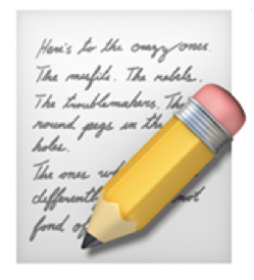
\includegraphics[height=10pt]{graphs/write.png}
                \newline
                    (193) Concise, conversational, and whimsical bullet-point summaries with emojis. 
\includegraphics[height=10pt]{graphs/tada.png} 
\includegraphics[height=10pt]{graphs/sparkles.png} 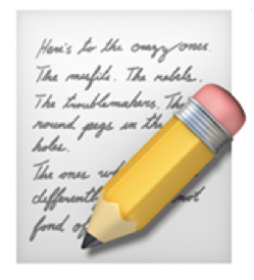
\includegraphics[height=10pt]{graphs/write.png} 
\includegraphics[height=10pt]{graphs/rocket.png} \\
        \midrule
        \textbf{Movie review.} question answering style & (12) The user prefers a straightforward, clear, and concise writing style with factual formatting.
        \newline (123) The user prefers a clear and concise question and answer format with straightforward language. 
        \newline (199) Concise, Structured Q\&A with Whimsical Clarity \\
            
                
               
        \bottomrule
    \end{tabular} 
    \label{tab:learned_prefs}
\end{table}










